% Options for packages loaded elsewhere
\PassOptionsToPackage{unicode}{hyperref}
\PassOptionsToPackage{hyphens}{url}
%
\documentclass[
  ignorenonframetext,
  aspectratio=169,
]{beamer}
\usepackage{pgfpages}
\setbeamertemplate{caption}[numbered]
\setbeamertemplate{caption label separator}{: }
\setbeamercolor{caption name}{fg=normal text.fg}
\beamertemplatenavigationsymbolsempty
% Prevent slide breaks in the middle of a paragraph
\widowpenalties 1 10000
\raggedbottom
\setbeamertemplate{part page}{
  \centering
  \begin{beamercolorbox}[sep=16pt,center]{part title}
    \usebeamerfont{part title}\insertpart\par
  \end{beamercolorbox}
}
\setbeamertemplate{section page}{
  \centering
  \begin{beamercolorbox}[sep=12pt,center]{part title}
    \usebeamerfont{section title}\insertsection\par
  \end{beamercolorbox}
}
\setbeamertemplate{subsection page}{
  \centering
  \begin{beamercolorbox}[sep=8pt,center]{part title}
    \usebeamerfont{subsection title}\insertsubsection\par
  \end{beamercolorbox}
}
\AtBeginPart{
  \frame{\partpage}
}
\AtBeginSection{
  \ifbibliography
  \else
    \frame{\sectionpage}
  \fi
}
\AtBeginSubsection{
  \frame{\subsectionpage}
}

\usepackage{amsmath,amssymb}
\usepackage{iftex}
\ifPDFTeX
  \usepackage[T1]{fontenc}
  \usepackage[utf8]{inputenc}
  \usepackage{textcomp} % provide euro and other symbols
\else % if luatex or xetex
  \usepackage{unicode-math}
  \defaultfontfeatures{Scale=MatchLowercase}
  \defaultfontfeatures[\rmfamily]{Ligatures=TeX,Scale=1}
\fi
\usepackage{lmodern}
\usetheme[progressbar=frametitle,sectionpage=progressbar,numbering=fraction]{metropolis}
\ifPDFTeX\else  
    % xetex/luatex font selection
\fi
% Use upquote if available, for straight quotes in verbatim environments
\IfFileExists{upquote.sty}{\usepackage{upquote}}{}
\IfFileExists{microtype.sty}{% use microtype if available
  \usepackage[]{microtype}
  \UseMicrotypeSet[protrusion]{basicmath} % disable protrusion for tt fonts
}{}
\makeatletter
\@ifundefined{KOMAClassName}{% if non-KOMA class
  \IfFileExists{parskip.sty}{%
    \usepackage{parskip}
  }{% else
    \setlength{\parindent}{0pt}
    \setlength{\parskip}{6pt plus 2pt minus 1pt}}
}{% if KOMA class
  \KOMAoptions{parskip=half}}
\makeatother
\usepackage{xcolor}
\newif\ifbibliography
\setlength{\emergencystretch}{3em} % prevent overfull lines
\setcounter{secnumdepth}{5}


\providecommand{\tightlist}{%
  \setlength{\itemsep}{0pt}\setlength{\parskip}{0pt}}\usepackage{longtable,booktabs,array}
\usepackage{calc} % for calculating minipage widths
\usepackage{caption}
% Make caption package work with longtable
\makeatletter
\def\fnum@table{\tablename~\thetable}
\makeatother
\usepackage{graphicx}
\makeatletter
\def\maxwidth{\ifdim\Gin@nat@width>\linewidth\linewidth\else\Gin@nat@width\fi}
\def\maxheight{\ifdim\Gin@nat@height>\textheight\textheight\else\Gin@nat@height\fi}
\makeatother
% Scale images if necessary, so that they will not overflow the page
% margins by default, and it is still possible to overwrite the defaults
% using explicit options in \includegraphics[width, height, ...]{}
\setkeys{Gin}{width=\maxwidth,height=\maxheight,keepaspectratio}
% Set default figure placement to htbp
\makeatletter
\def\fps@figure{htbp}
\makeatother

\makeatletter
\@ifpackageloaded{caption}{}{\usepackage{caption}}
\AtBeginDocument{%
\ifdefined\contentsname
  \renewcommand*\contentsname{Содержание}
\else
  \newcommand\contentsname{Содержание}
\fi
\ifdefined\listfigurename
  \renewcommand*\listfigurename{Список иллюстраций}
\else
  \newcommand\listfigurename{Список иллюстраций}
\fi
\ifdefined\listtablename
  \renewcommand*\listtablename{Список таблиц}
\else
  \newcommand\listtablename{Список таблиц}
\fi
\ifdefined\figurename
  \renewcommand*\figurename{Рисунок}
\else
  \newcommand\figurename{Рисунок}
\fi
\ifdefined\tablename
  \renewcommand*\tablename{Таблица}
\else
  \newcommand\tablename{Таблица}
\fi
}
\@ifpackageloaded{float}{}{\usepackage{float}}
\floatstyle{ruled}
\@ifundefined{c@chapter}{\newfloat{codelisting}{h}{lop}}{\newfloat{codelisting}{h}{lop}[chapter]}
\floatname{codelisting}{Список}
\newcommand*\listoflistings{\listof{codelisting}{Листинги}}
\makeatother
\makeatletter
\makeatother
\makeatletter
\@ifpackageloaded{caption}{}{\usepackage{caption}}
\@ifpackageloaded{subcaption}{}{\usepackage{subcaption}}
\makeatother
\ifLuaTeX
\usepackage[bidi=basic]{babel}
\else
\usepackage[bidi=default]{babel}
\fi
\babelprovide[main,import]{russian}
\babelprovide[import]{english}
% get rid of language-specific shorthands (see #6817):
\let\LanguageShortHands\languageshorthands
\def\languageshorthands#1{}
\ifLuaTeX
  \usepackage{selnolig}  % disable illegal ligatures
\fi
\usepackage{bookmark}

\IfFileExists{xurl.sty}{\usepackage{xurl}}{} % add URL line breaks if available
\urlstyle{same} % disable monospaced font for URLs
\hypersetup{
  pdftitle={Презентация к лабораторной работе 1},
  pdfauthor={Власов Артем Сергеевич},
  pdflang={ru-RU},
  hidelinks,
  pdfcreator={LaTeX via pandoc}}

\title{Презентация к лабораторной работе 1}
\subtitle{Власов Артем Сергеевич}
\author{Власов Артем Сергеевич}
\date{2025-06-09}

\begin{document}
\frame{\titlepage}

\renewcommand*\contentsname{Содержание}
\begin{frame}[allowframebreaks]
  \frametitle{Содержание}
  \tableofcontents[hideallsubsections]
\end{frame}
\begin{frame}{1. Информация}
\phantomsection\label{ux438ux43dux444ux43eux440ux43cux430ux446ux438ux44f}
\begin{block}{1.1 Докладчик}
\phantomsection\label{ux434ux43eux43aux43bux430ux434ux447ux438ux43a}
\begin{columns}[c]
\begin{itemize}
\tightlist
\item
  Власов Артем Сергеевич
\item
  Группа НПИбд-01-24
\item
  Студент
\item
  Российский университет дружбы народов
\item
  \href{mailto:1132246841@pfur.ru}{\nolinkurl{1132246841@pfur.ru}}
\end{itemize}
\end{columns}
\end{block}

\begin{block}{1.2 Цели и задачи}
\phantomsection\label{ux446ux435ux43bux438-ux438-ux437ux430ux434ux430ux447ux438}
::: Установить Rocky Linux на виртуальную машину. :::
\end{block}
\end{frame}

\begin{frame}{2. Задание}
\phantomsection\label{ux437ux430ux434ux430ux43dux438ux435}
::: Установить и настроить опреационную систему, выполнить задание и
ответить на контрольные вопросы :::

\begin{block}{2.1 Создадим новую виртуальную машину с помощью файла
образа.}
\phantomsection\label{ux441ux43eux437ux434ux430ux434ux438ux43c-ux43dux43eux432ux443ux44e-ux432ux438ux440ux442ux443ux430ux43bux44cux43dux443ux44e-ux43cux430ux448ux438ux43dux443-ux441-ux43fux43eux43cux43eux449ux44cux44e-ux444ux430ux439ux43bux430-ux43eux431ux440ux430ux437ux430.}
\begin{columns}[c]
\begin{figure}

{\centering 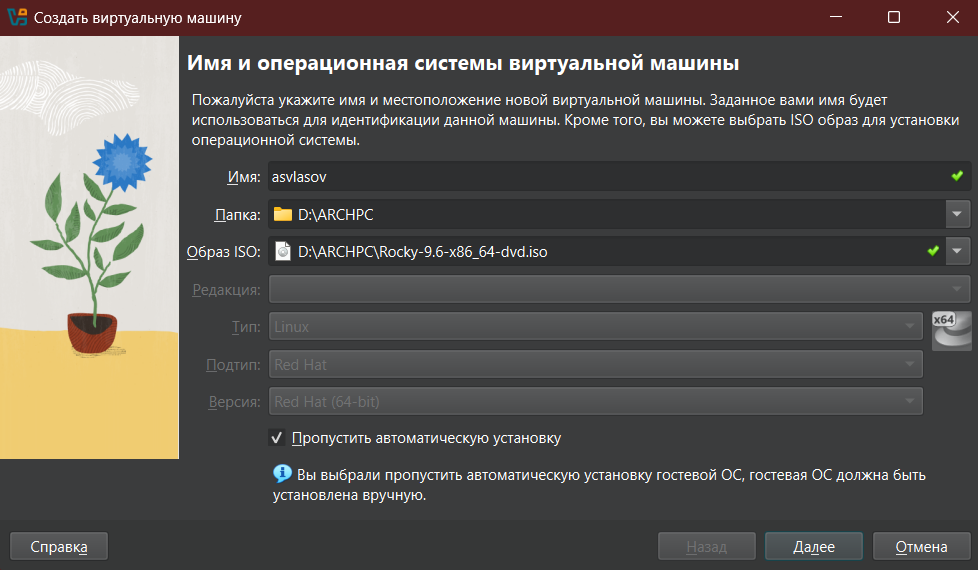
\includegraphics[width=0.7\textwidth,height=\textheight]{image/1.png}

}

\caption{Подключение образа}

\end{figure}%
\end{columns}
\end{block}

\begin{block}{2.2 Задаем первичные настройки машины.}
\phantomsection\label{ux437ux430ux434ux430ux435ux43c-ux43fux435ux440ux432ux438ux447ux43dux44bux435-ux43dux430ux441ux442ux440ux43eux439ux43aux438-ux43cux430ux448ux438ux43dux44b.}
\begin{columns}[c]
\begin{figure}

{\centering 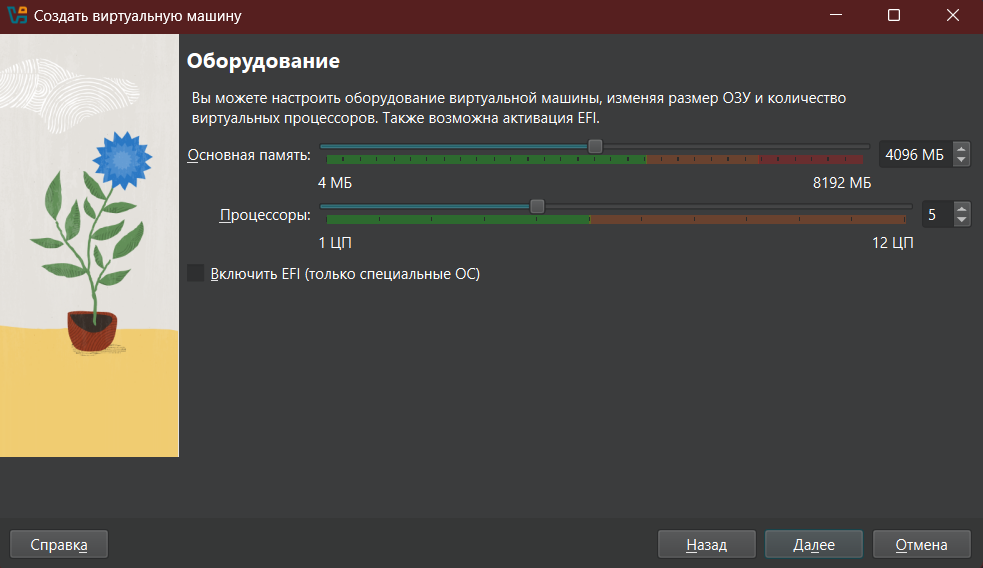
\includegraphics[width=0.7\textwidth,height=\textheight]{image/2.png}

}

\caption{Настраиваем ОЗУ и ядра процессора}

\end{figure}%%
\begin{figure}

{\centering 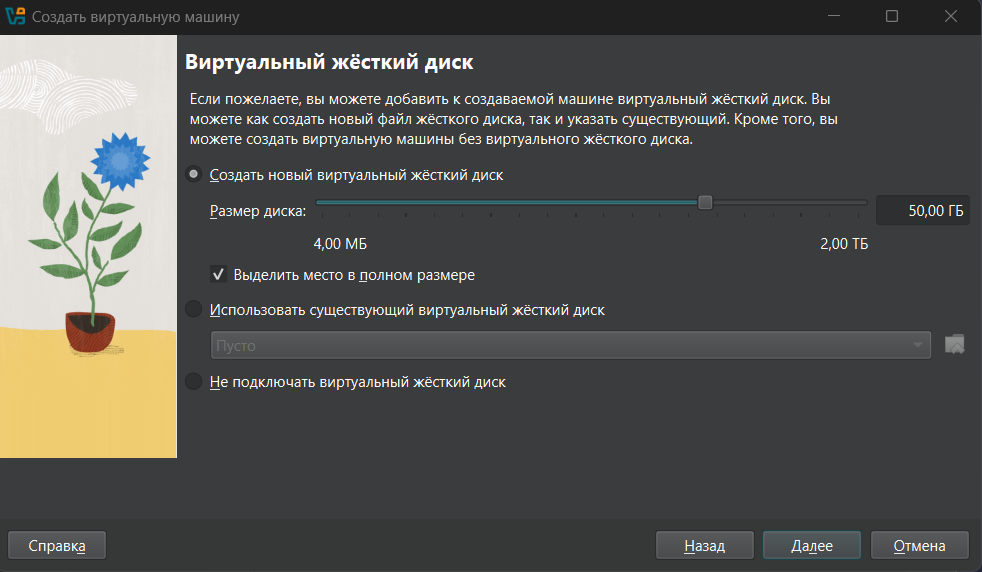
\includegraphics[width=0.7\textwidth,height=\textheight]{image/3.png}

}

\caption{Добавляем виртуальный диск}

\end{figure}%
\end{columns}
\end{block}

\begin{block}{2.3 Запуск и настройка ОС.}
\phantomsection\label{ux437ux430ux43fux443ux441ux43a-ux438-ux43dux430ux441ux442ux440ux43eux439ux43aux430-ux43eux441.}
\begin{columns}[c]
\begin{figure}

{\centering 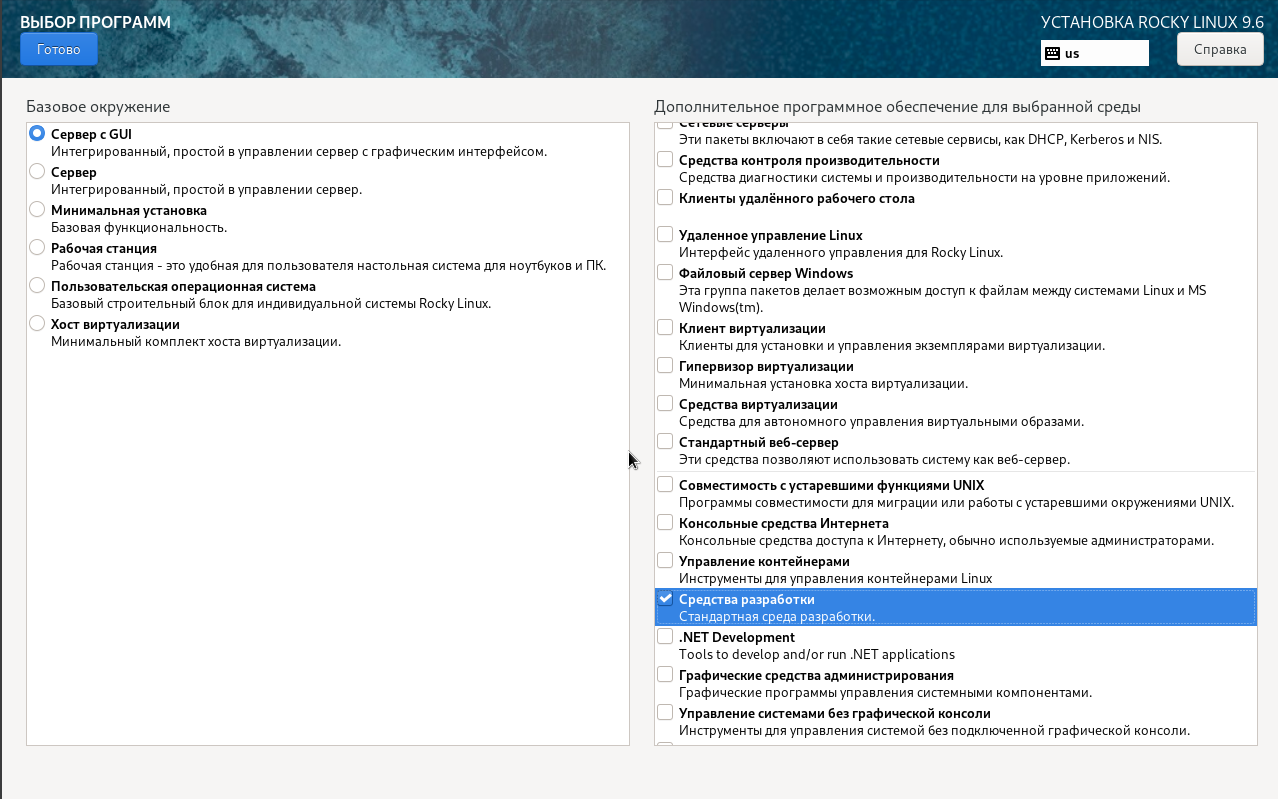
\includegraphics[width=0.7\textwidth,height=\textheight]{image/6.png}

}

\caption{Добавление стандартных утилит}

\end{figure}%%
\begin{figure}

{\centering 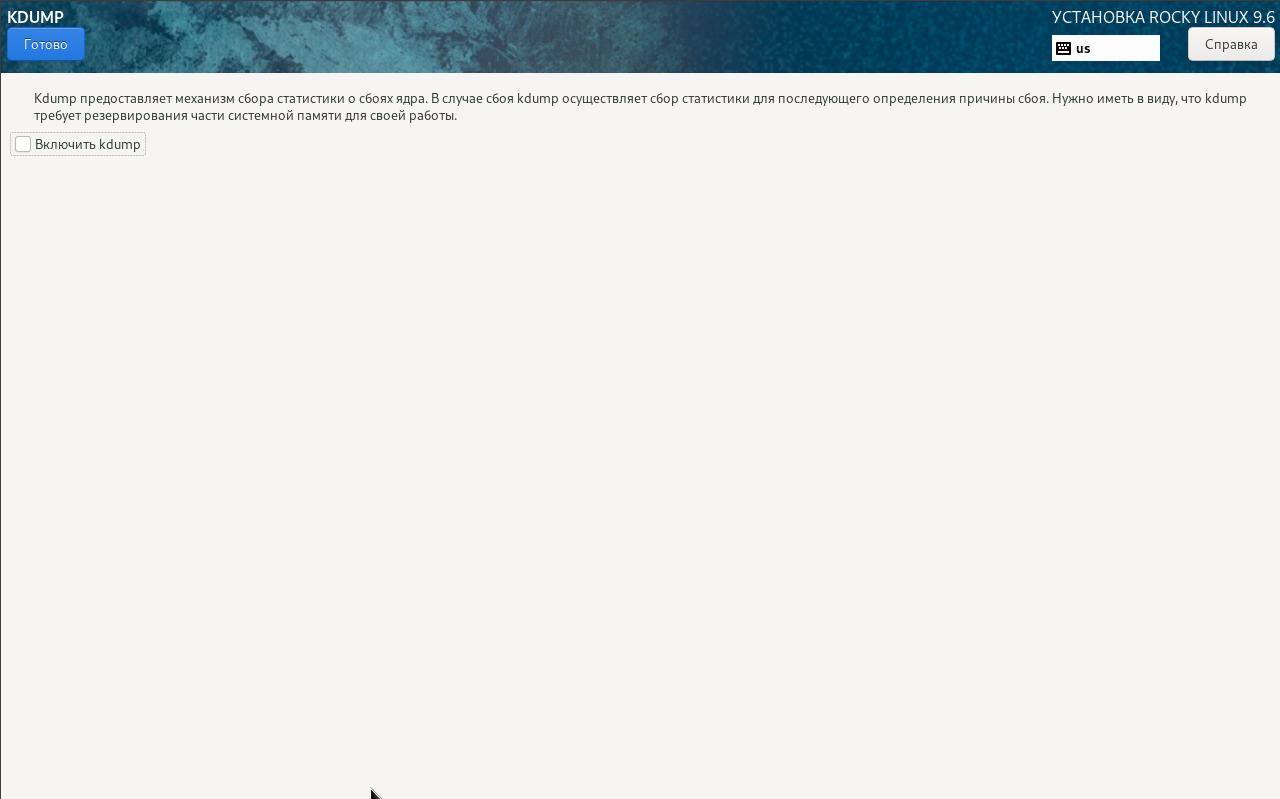
\includegraphics[width=0.7\textwidth,height=\textheight]{image/7.png}

}

\caption{Отключение KDUMP}

\end{figure}%
\end{columns}
\end{block}

\begin{block}{2.4 Запуск и настройка ОС.}
\phantomsection\label{ux437ux430ux43fux443ux441ux43a-ux438-ux43dux430ux441ux442ux440ux43eux439ux43aux430-ux43eux441.-1}
\begin{columns}[c]
\begin{figure}

{\centering 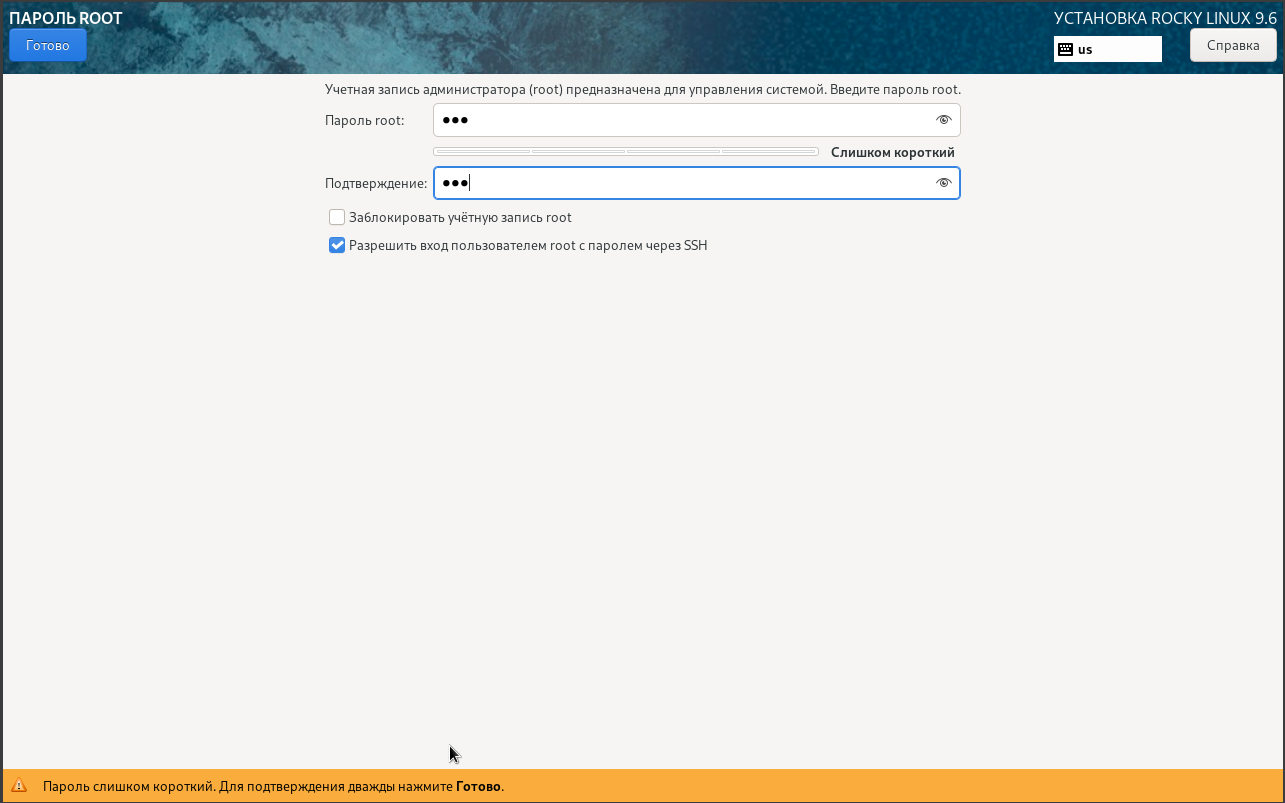
\includegraphics[width=0.7\textwidth,height=\textheight]{image/10.png}

}

\caption{ROOT}

\end{figure}%%
\begin{figure}

{\centering 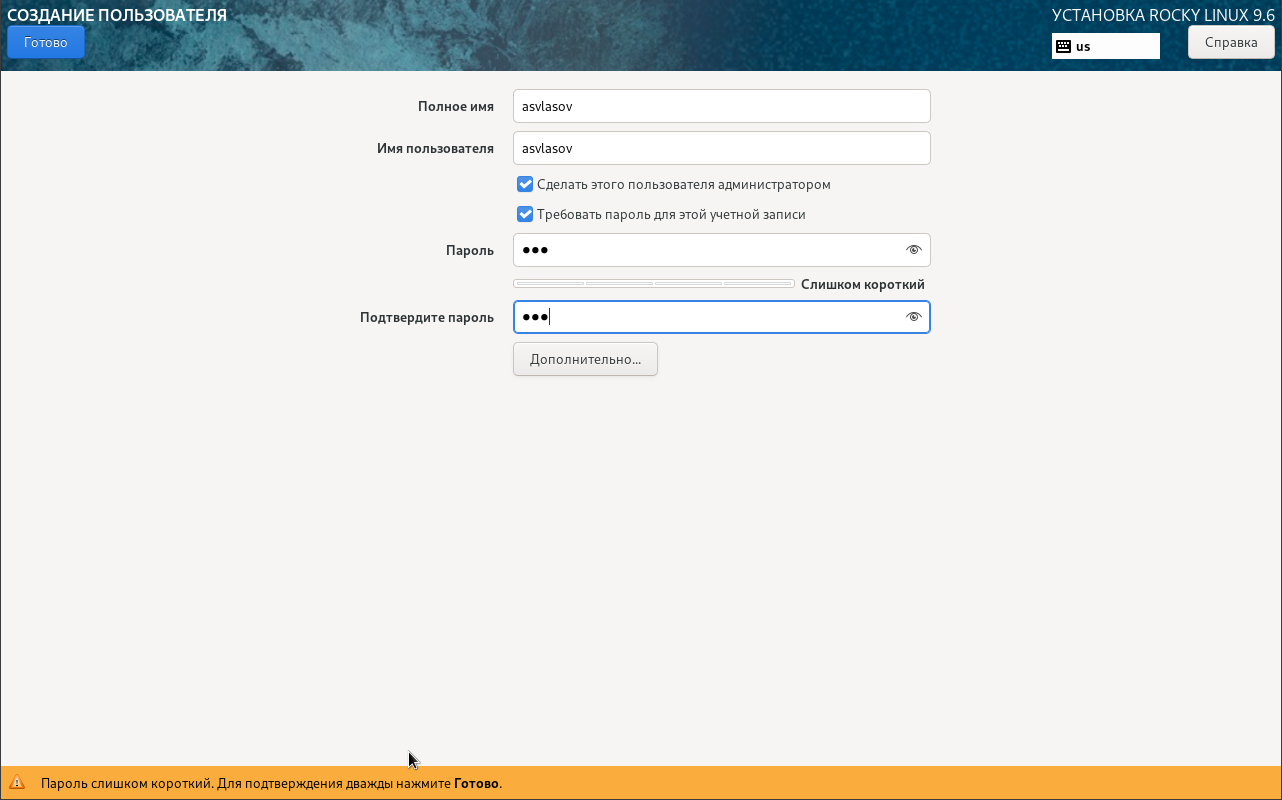
\includegraphics[width=0.7\textwidth,height=\textheight]{image/11.png}

}

\caption{Настройка пользователя}

\end{figure}%
\end{columns}
\end{block}

\begin{block}{2.5 Запуск и настройка ОС.}
\phantomsection\label{ux437ux430ux43fux443ux441ux43a-ux438-ux43dux430ux441ux442ux440ux43eux439ux43aux430-ux43eux441.-2}
\begin{columns}[c]
\begin{figure}

{\centering 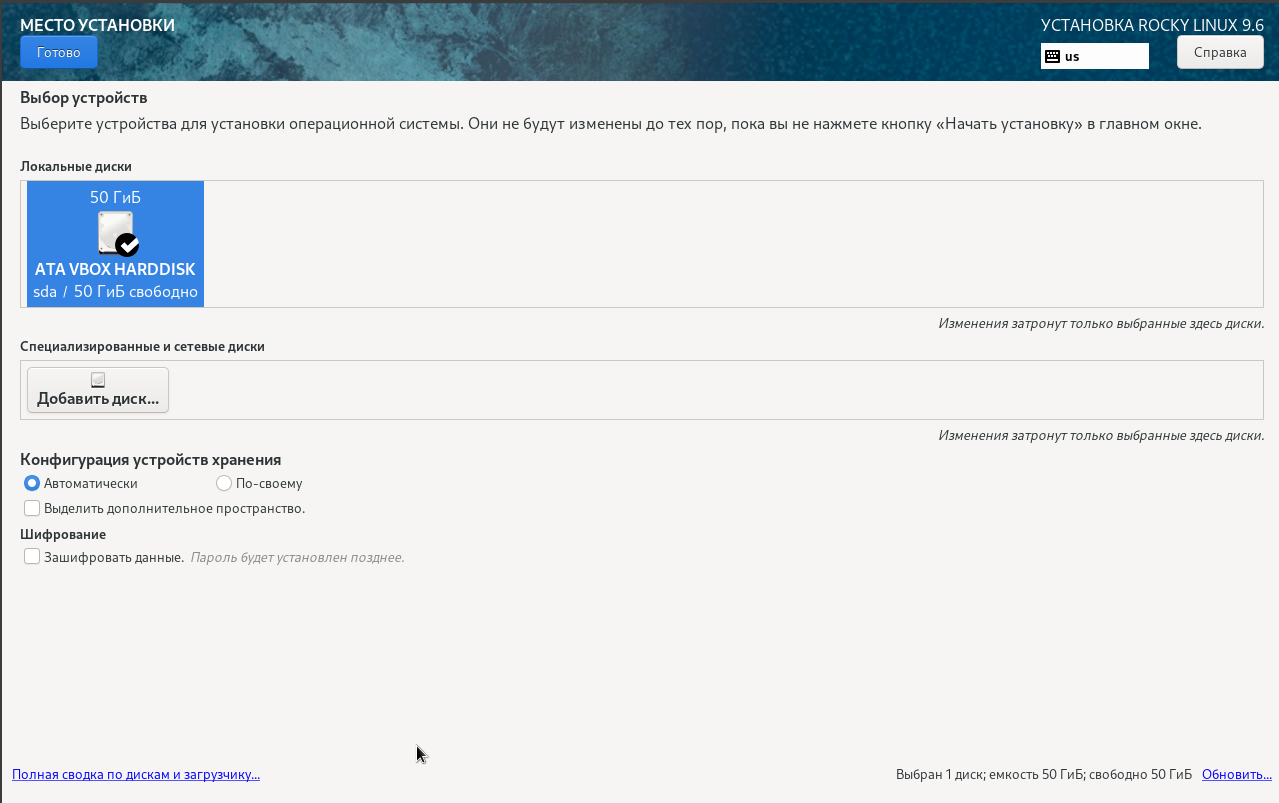
\includegraphics[width=0.7\textwidth,height=\textheight]{image/8.png}

}

\caption{Добавление диска}

\end{figure}%%
\begin{figure}

{\centering 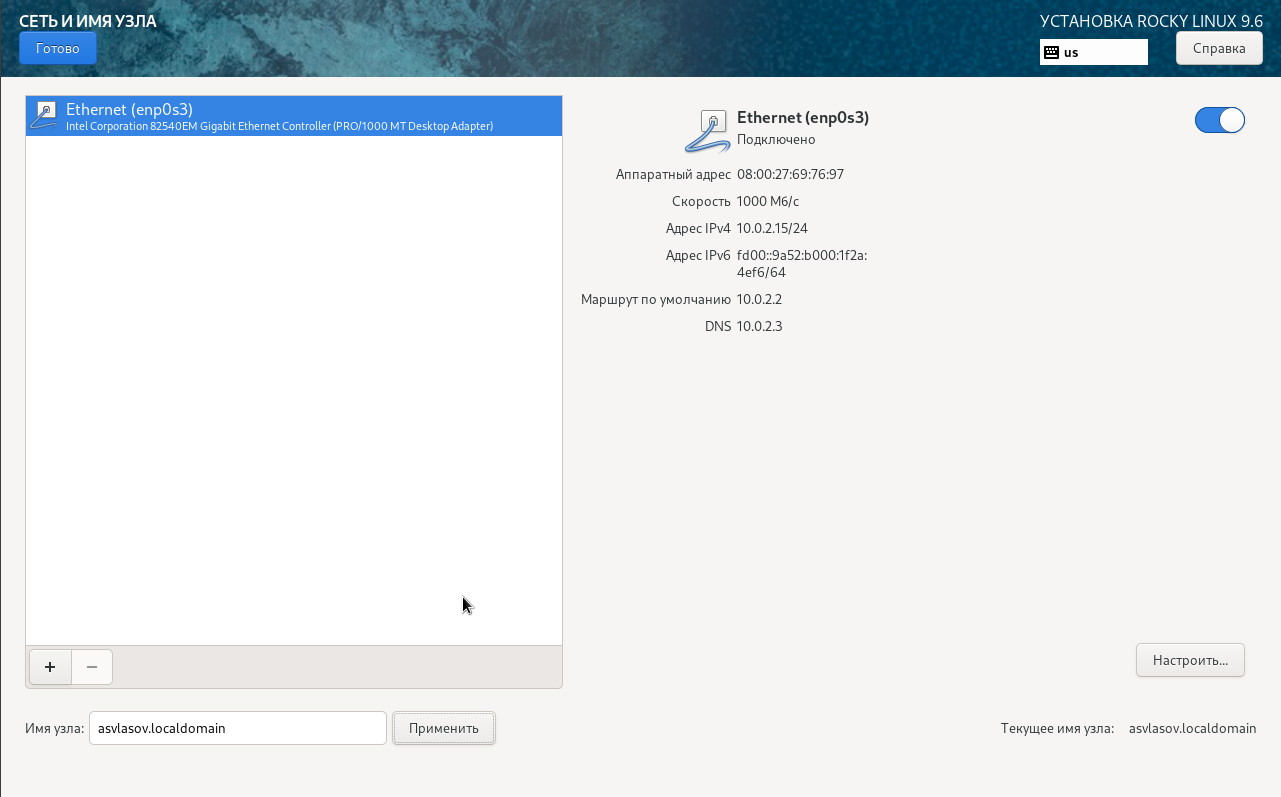
\includegraphics[width=0.7\textwidth,height=\textheight]{image/9.png}

}

\caption{Настройка сети}

\end{figure}%
\end{columns}
\end{block}

\begin{block}{2.6 Запуск и настройка ОС.}
\phantomsection\label{ux437ux430ux43fux443ux441ux43a-ux438-ux43dux430ux441ux442ux440ux43eux439ux43aux430-ux43eux441.-3}
\begin{columns}[c]
\begin{figure}

{\centering 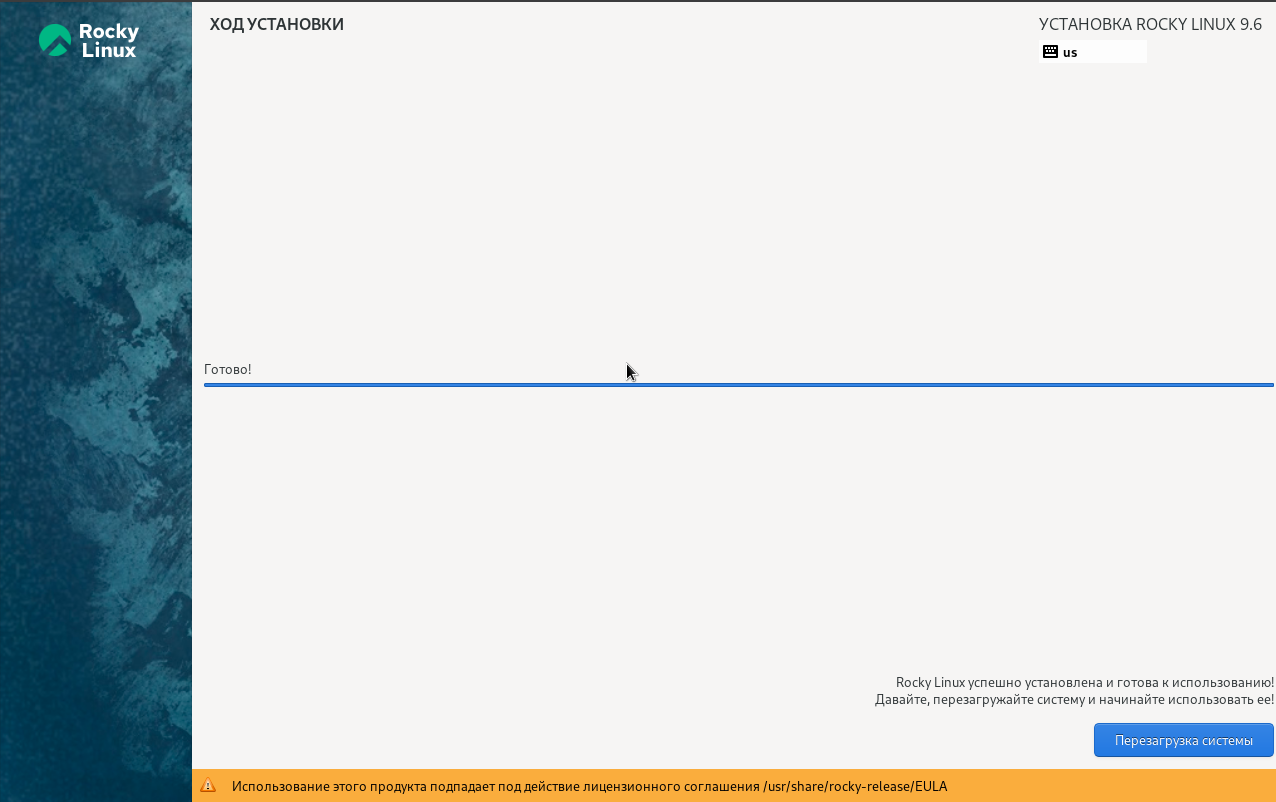
\includegraphics[width=0.7\textwidth,height=\textheight]{image/13.png}

}

\caption{Завершение установки}

\end{figure}%%
\begin{figure}

{\centering 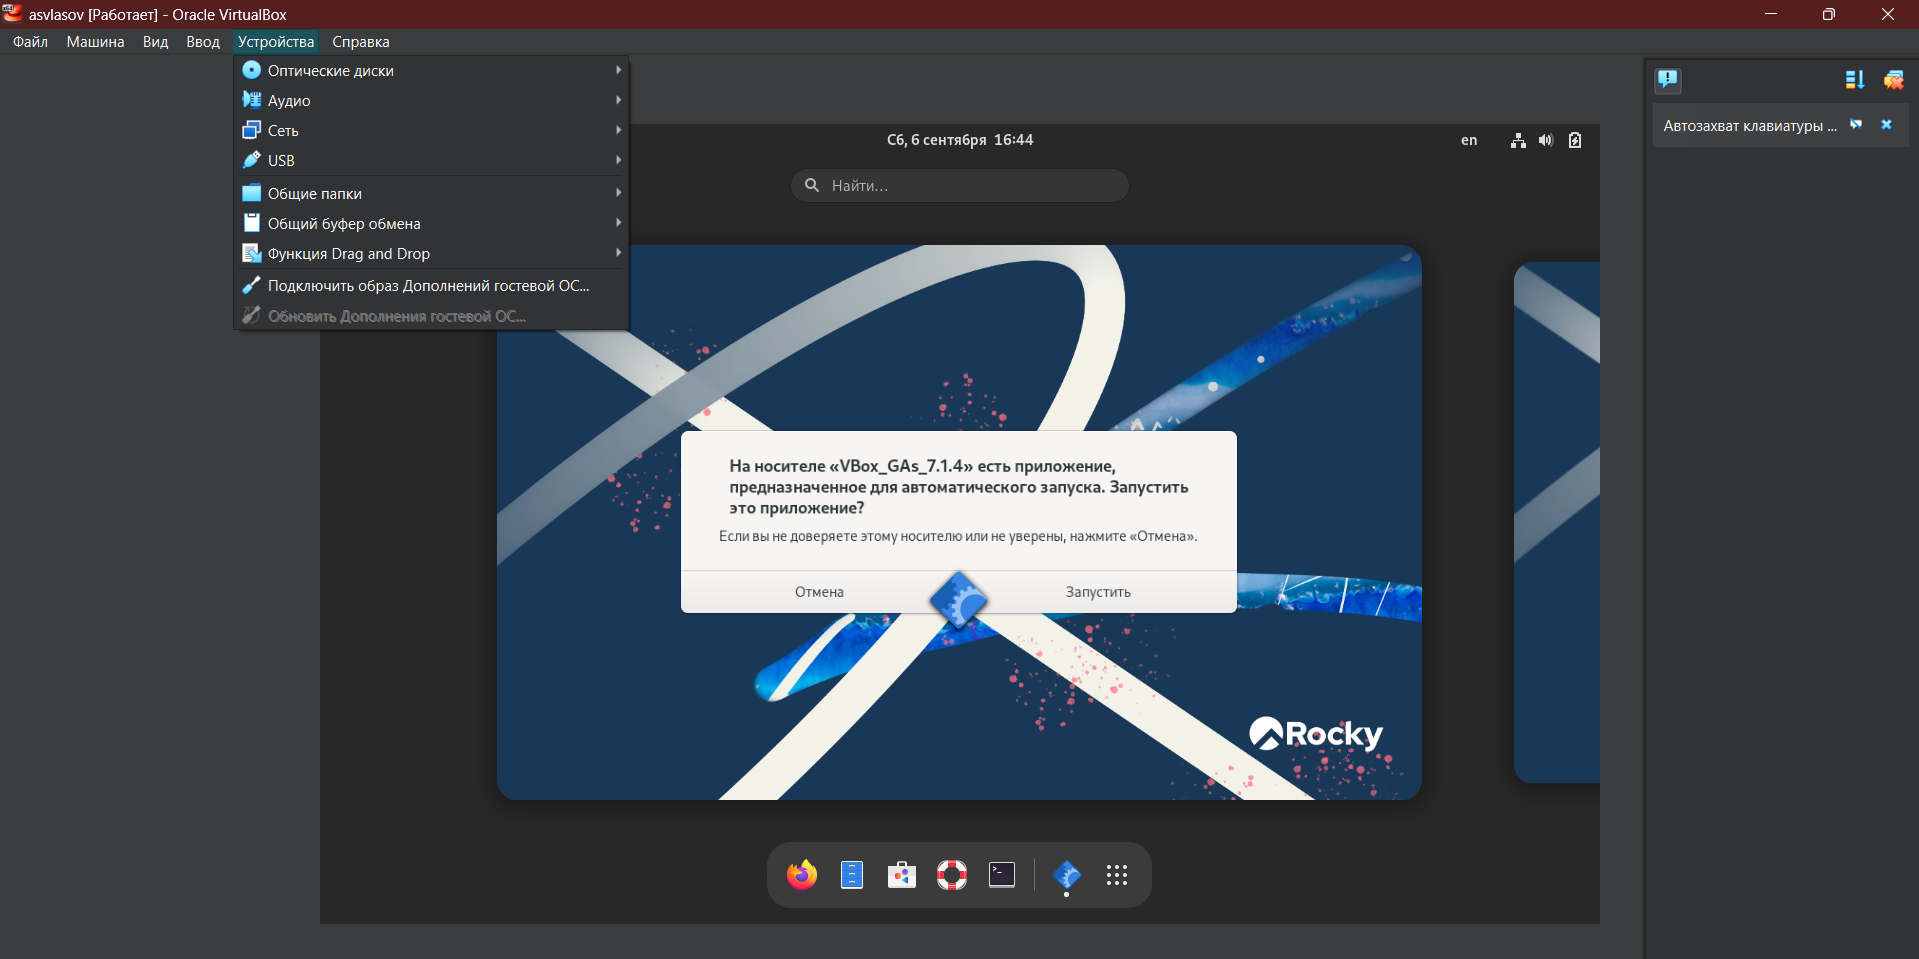
\includegraphics[width=0.7\textwidth,height=\textheight]{image/14.png}

}

\caption{Подключение образа дополнений гостевой ОС}

\end{figure}%
\end{columns}
\end{block}

\begin{block}{2.7 Выполение домашнего задания}
\phantomsection\label{ux432ux44bux43fux43eux43bux435ux43dux438ux435-ux434ux43eux43cux430ux448ux43dux435ux433ux43e-ux437ux430ux434ux430ux43dux438ux44f}
\begin{columns}[c]
\begin{figure}

{\centering 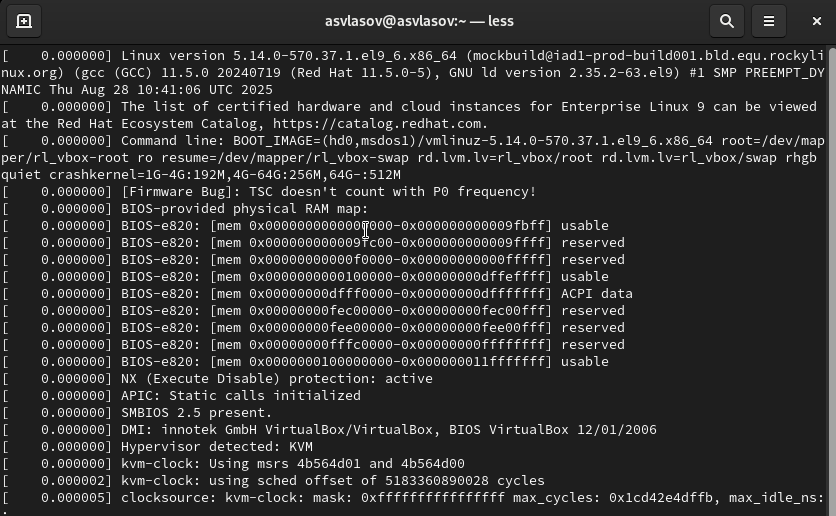
\includegraphics[width=0.7\textwidth,height=\textheight]{image/16.png}

}

\caption{Команда для просмотра технических характеристик}

\end{figure}%
\end{columns}
\end{block}

\begin{block}{2.8 Выполение домашнего задания}
\phantomsection\label{ux432ux44bux43fux43eux43bux435ux43dux438ux435-ux434ux43eux43cux430ux448ux43dux435ux433ux43e-ux437ux430ux434ux430ux43dux438ux44f-1}
\begin{columns}[c]
\begin{figure}

{\centering 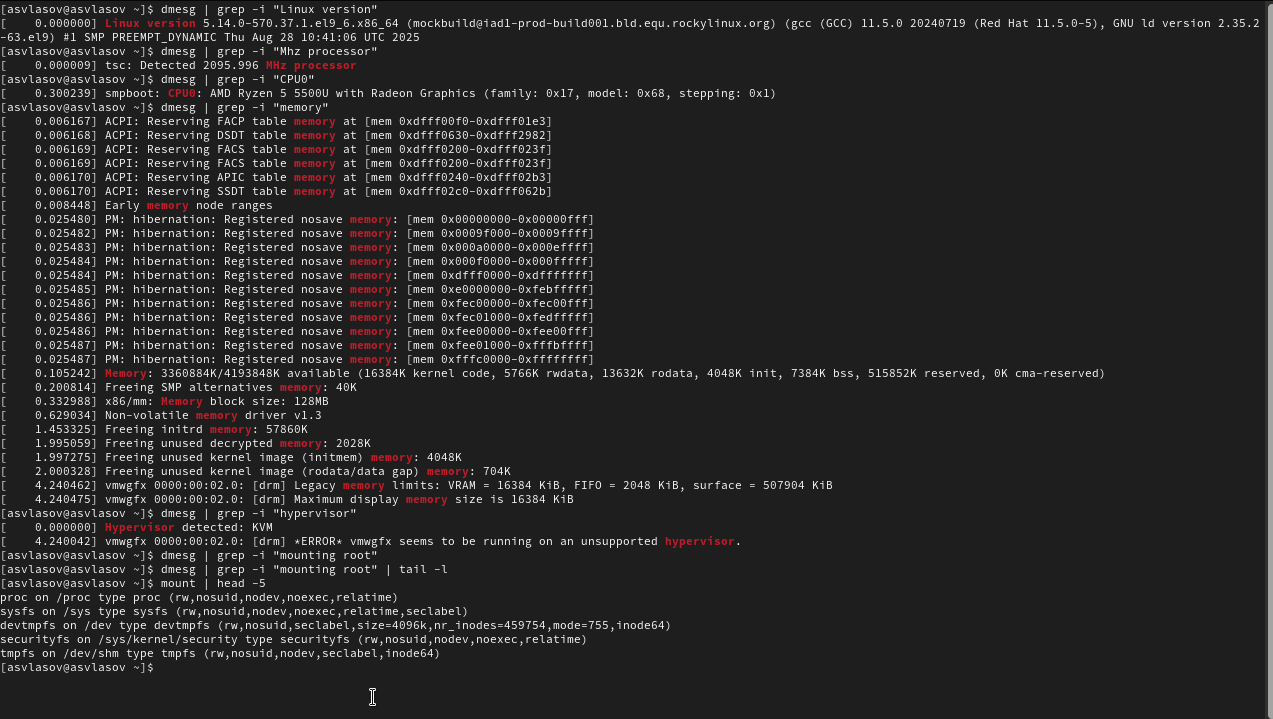
\includegraphics[width=0.7\textwidth,height=\textheight]{image/17.png}

}

\caption{Поиск семи элементов в тех. характеристиках}

\end{figure}%
\end{columns}
\end{block}

\begin{block}{2.9 Выводы}
\phantomsection\label{ux432ux44bux432ux43eux434ux44b}
Мы установили ОС на виртуальную машину, выполнили задание и ответили на
контрольные вопросы.
\end{block}
\end{frame}



\end{document}
